\documentclass{article}
\usepackage{graphicx} % Required for inserting images
\usepackage{tikz}
\usepackage{float}
\usepackage{amsmath}
\usepackage{amsthm}

\title{$\aleph_{0}$ Weekly Problem}
\author{Ravi Dayabhai \& Conrad Warren}
\date{2024-08-07}

\begin{document}
\maketitle

\section*{Problem}

Show that there do not exist any equilateral triangles in the plane whose vertices are lattice points (integer coordinates).

\section*{Solution}

\begin{proof}

We will attempt to construct an equilateral triangle in the plane whose vertices are all lattice points (i.e., having integer coordinates), but show that this is impossible, thereby, demonstrating no such triangle can exist.

We start by fixing one vertex $v_{1}$ at point $(0, 0)$, the second $v_{2}$ at point $(\frac{\sqrt{3}r}{2}, 0)$, and the third $v_{3}$ at $(\frac{\sqrt{3}r}{2}, \frac{3}{2}r)$, yielding an equilateral triangle having side lengths equal to $\sqrt{3}r$ (notionally circumscribed by a circle centered at $(\frac{\sqrt{3}}{2}r, \frac{1}{2}r)$ having radius $r$).

\begin{figure}[H]
    \centering
    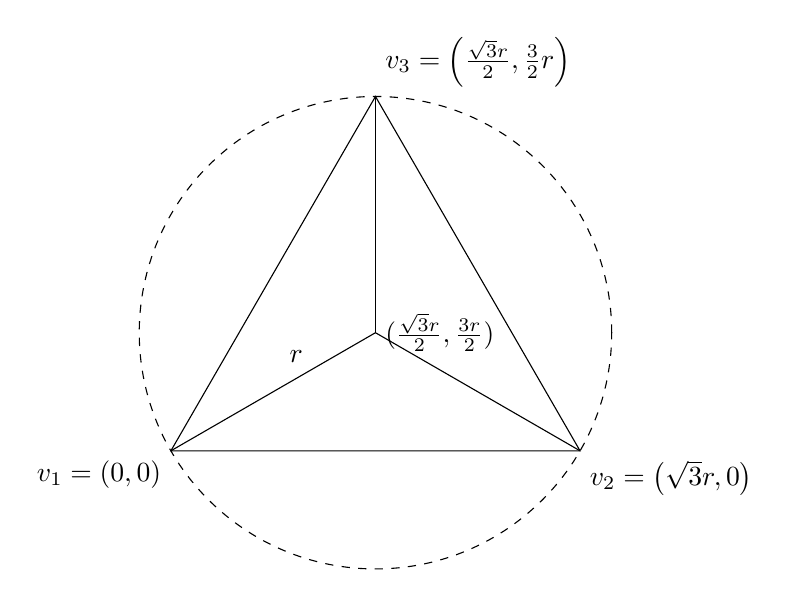
\begin{tikzpicture}
        % Define the radius r
        \def\r{3}
    
        % Calculate the coordinates
        \coordinate (V_1) at (0, 0);
        \coordinate (V_3) at ({sqrt(3)*\r/2}, {3*\r/2});
        \coordinate (O) at ({sqrt(3)*\r/2}, {\r/2}); % Center of the circle
        \coordinate (V_2) at ({sqrt(3)*\r}, 0);

        
        % Draw the triangle
        \draw (V_1) -- (V_2) -- (V_3) -- cycle;
        \draw (O) -- (V_1);
        \draw (O) -- (V_2);
        \draw (O) -- (V_3);
        
        % Draw the circumscribed circle
        \draw[dashed] (O) circle (\r);
        
        % Label the vertices
        \node[right] at (O) {$(\frac{\sqrt{3}r}{2}, \frac{3r}{2})$};
        \node[below left] at (V_1) {$v_1 = (0, 0)$};
        \node[above right] at (V_3) {$v_3 = \left(\frac{\sqrt{3}r}{2}, \frac{3}{2}r\right)$};
        \node[below right] at (V_2) {$v_2 = \left(\sqrt{3}r, 0\right)$};   
        
        \node[left] at (1.8, 1.2) {$r$};
    \end{tikzpicture}
    \caption{Equilateral triangle with side length \(\sqrt{3}r\)}
    \label{fig:fig1}
\end{figure}

Note that we can scale the triangle by $r$ and rotate the triangle about $v_{1}$ by some angle $\theta$ between the $v_{1}$--$v_{2}$ side of the triangle and the $x$-axis, as seen in figure \ref{fig:fig2}.

Treating $v_{2}$ and $v_{3}$ as vectors allows us to perform any scaling and rotation. With $v_{1}$ fixed, we can express the new coordinates of the triangle's vertices under any scaling and rotation as:

\begin{align*}
    v^{\prime}_{1} &= v_{1} =
        \begin{bmatrix}
            0\\
            0
        \end{bmatrix}\\
    v^{\prime}_{2} &= 
        \begin{bmatrix}
            \cos{\theta} & -\sin{\theta}\\
            \sin{\theta} & \cos{\theta}
        \end{bmatrix}
        \begin{bmatrix}
            \sqrt{3}r\\
            0
        \end{bmatrix}
        = 
        \begin{bmatrix}
            \sqrt{3}r\cos{\theta}\\
            \sqrt{3}r\sin{\theta}
        \end{bmatrix} \\
    v^{\prime}_{3} &= 
        \begin{bmatrix}
            \cos{\theta} & -\sin{\theta}\\
            \sin{\theta} & \cos{\theta}
        \end{bmatrix}
        \begin{bmatrix}
            \frac{\sqrt{3}r}{2}\\
            \frac{3r}{2}
        \end{bmatrix}
        = 
        \begin{bmatrix}
            \frac{\sqrt{3}r}{2}\cos{\theta} - \frac{3r}{2}\sin{\theta}\\
            \frac{\sqrt{3}r}{2}\sin{\theta} + \frac{3r}{2}\cos{\theta}
        \end{bmatrix}
\end{align*}

If we let $A = \sqrt{3}r\cos{\theta}$ and $B = \sqrt{3}r\sin{\theta}$, we get:

\begin{align*}
    v^{\prime}_{2} &= 
        \begin{bmatrix}
            A\\
            B
        \end{bmatrix} \\
    v^{\prime}_{3} &= 
        \begin{bmatrix}
            \frac{A}{2} - \frac{B\sqrt{3}}{2}\\
            \frac{B}{2} - \frac{A\sqrt{3}}{2}\\
        \end{bmatrix}
\end{align*}

\begin{figure}[H]
    \centering
    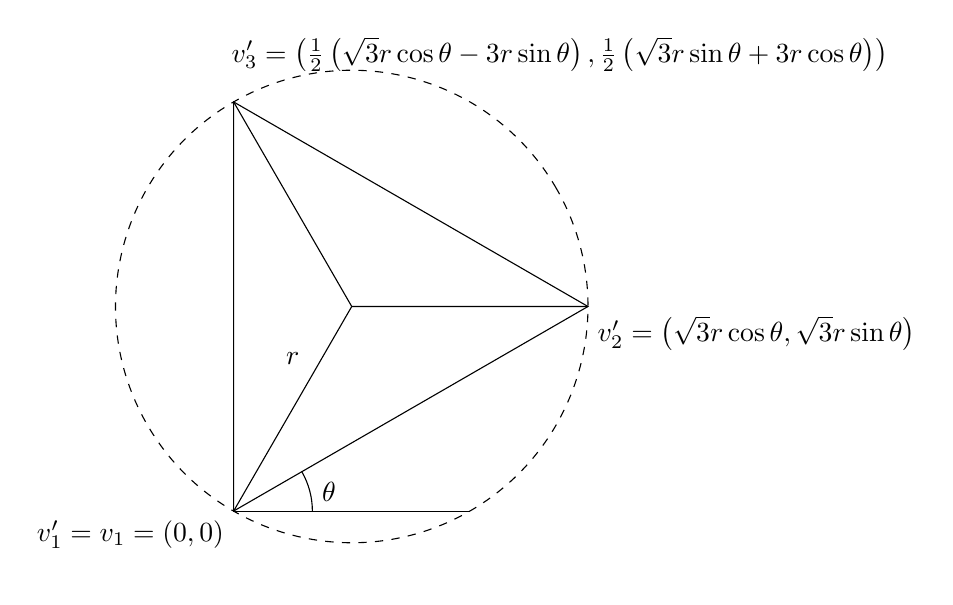
\begin{tikzpicture}
        % Define the radius r
        \def\r{3}
            \begin{scope}[rotate around={30:(0,0)}]
                 % Calculate the coordinates
            \coordinate (V_1) at (0, 0);
            \coordinate (V_3) at ({sqrt(3)*\r/2}, {3*\r/2});
            \coordinate (O) at ({sqrt(3)*\r/2}, {\r/2}); % Center of the circle
            \coordinate (V_2) at ({sqrt(3)*\r}, 0);
    
            
            % Draw the triangle
            \draw (V_1) -- (V_2) -- (V_3) -- cycle;
            \draw (O) -- (V_1);
            \draw (O) -- (V_2);
            \draw (O) -- (V_3);
            
            % Draw the circumscribed circle
            \draw[dashed] (O) circle (\r);
            
            % Label the vertices
    
            \node[below left] at (V_1) {$v^{\prime}_1 = v_1 = (0, 0)$};
            \node[above right] at ({sqrt(3)*\r/2}, {(3*\r/2) + 0.3}) {$v^{\prime}_3 = \left(\frac{1}{2}\left(\sqrt{3}r\cos\theta - 3r\sin\theta\right), \frac{1}{2}\left(\sqrt{3}r\sin\theta + 3r\cos\theta\right)\right)$};
            \node[below right] at (V_2) {$v^{\prime}_2 = \left(\sqrt{3}r\cos\theta, \sqrt{3}r\sin\theta \right)$};   
            
            \node[left] at (1.8, 1.2) {$r$};
        \end{scope}
            \coordinate (X) at (\r, 0);
            \draw (1,0) arc[start angle=0, end angle=30, radius=1cm];
            \draw (V_1) -- (X);
            \node[above right] at (1, 0) {$\theta$};
            
    \end{tikzpicture}
    \caption{Equilateral triangle rotated around point \((0,0)\)}
    \label{fig:fig2}
\end{figure}

But now we clearly see that not all four coordinates of $v^{\prime}_{2}$ and $v^{\prime}_{3}$ can be simultaneously integer-valued, since integer-valued coordinates of $v^{\prime}_{2}$ (i.e., $A$ and $B$) implies non-integer values for the coordinates of $v^{\prime}_{3}$: an irrational number (e.g., $\frac{B\sqrt{3}}{2}$) subtracted from a rational number (e.g., $\frac{A}{2}$) produces an irrational (e.g., $\frac{A}{2} - \frac{B\sqrt{3}}{2}$).

Since the choice of fixing $v_{1}$ was arbitrary, the above holds for any choice of integer-valued coordinates for $v_{1}$ (any non-integer valued coordinate for $v_{1}$ immediately violates the construction) because the addition of an integer-valued offset vector to each vertex doesn't change the fact that an irrational term will exist in at least one of the coordinates of $v^{\prime}_{2}$ or $v^{\prime}_{3}$.

\end{proof}

\end{document}